\chapter[O sistema]{O sistema}
Neste capítulo, são apresentados todos os componentes presentes no sistema,
 a configuração do ambiente de programação buscando padronizar as características para que possa ser aplicada e analisada por outro pesquisador.

\section{Contextualização}
  O principal incentivo em relação a esta proposta é fazer um produto que seja de ajuda
para a reabilitação motora  de indivíduos que apresentam deficiências motoras e ou físicas, que seja acessível e
que possa ser executada na hora que o paciente tiver disponibilidade.

  Com isso o sistema busca analisar o movimento de um índividuo com um movimento previamente
armazenado, dando \textit{feedbacks} em tempo real, para a correta execução. Além disso,
o sistema tem como objetivo a implementação de análise do movimento através da primeira
versão do \textit{kinect} por ser mais facilmente encontrado e por não gerar grandes custos, porém
sua precisão não é perfeita, sofrendo também de limitação por movimentos mais complexos.

Assim sendo, durante a primeira etapa deste trabalho,  foram estudadas algumas tecnologias para a implementação do sistema,
 ficou definido que seria usado o unity 3d para o desenvolvimento do sistema.

\subsection{Arquitetura}\label{sub:arquitetura}
  Podemos dividir o trabalho no unity em duas partes,
a primeira é a parte de vizualização, onde ele desponibiliza um espaço 3d para a inserção dos \textit{gameObjects} e criação das cenas. Um projeto pode
ter mais de uma cena e uma cena pode conter vários \textit{gameObjects}. A segunda é com os chamados \textit{scripts}, que são os códigos que podem
ser adicionados em um \textit{gameObject} dando-lhe a lógica de como se deve comportar durante uma cena de um projeto. Esses códigos podem ser escritos
nas linguagens \textit{javascript} e em C\#. Podemos ver uma representação da arquitetura em \ref{diagramaClasse}.


  \begin{figure}[H]
  \centering
  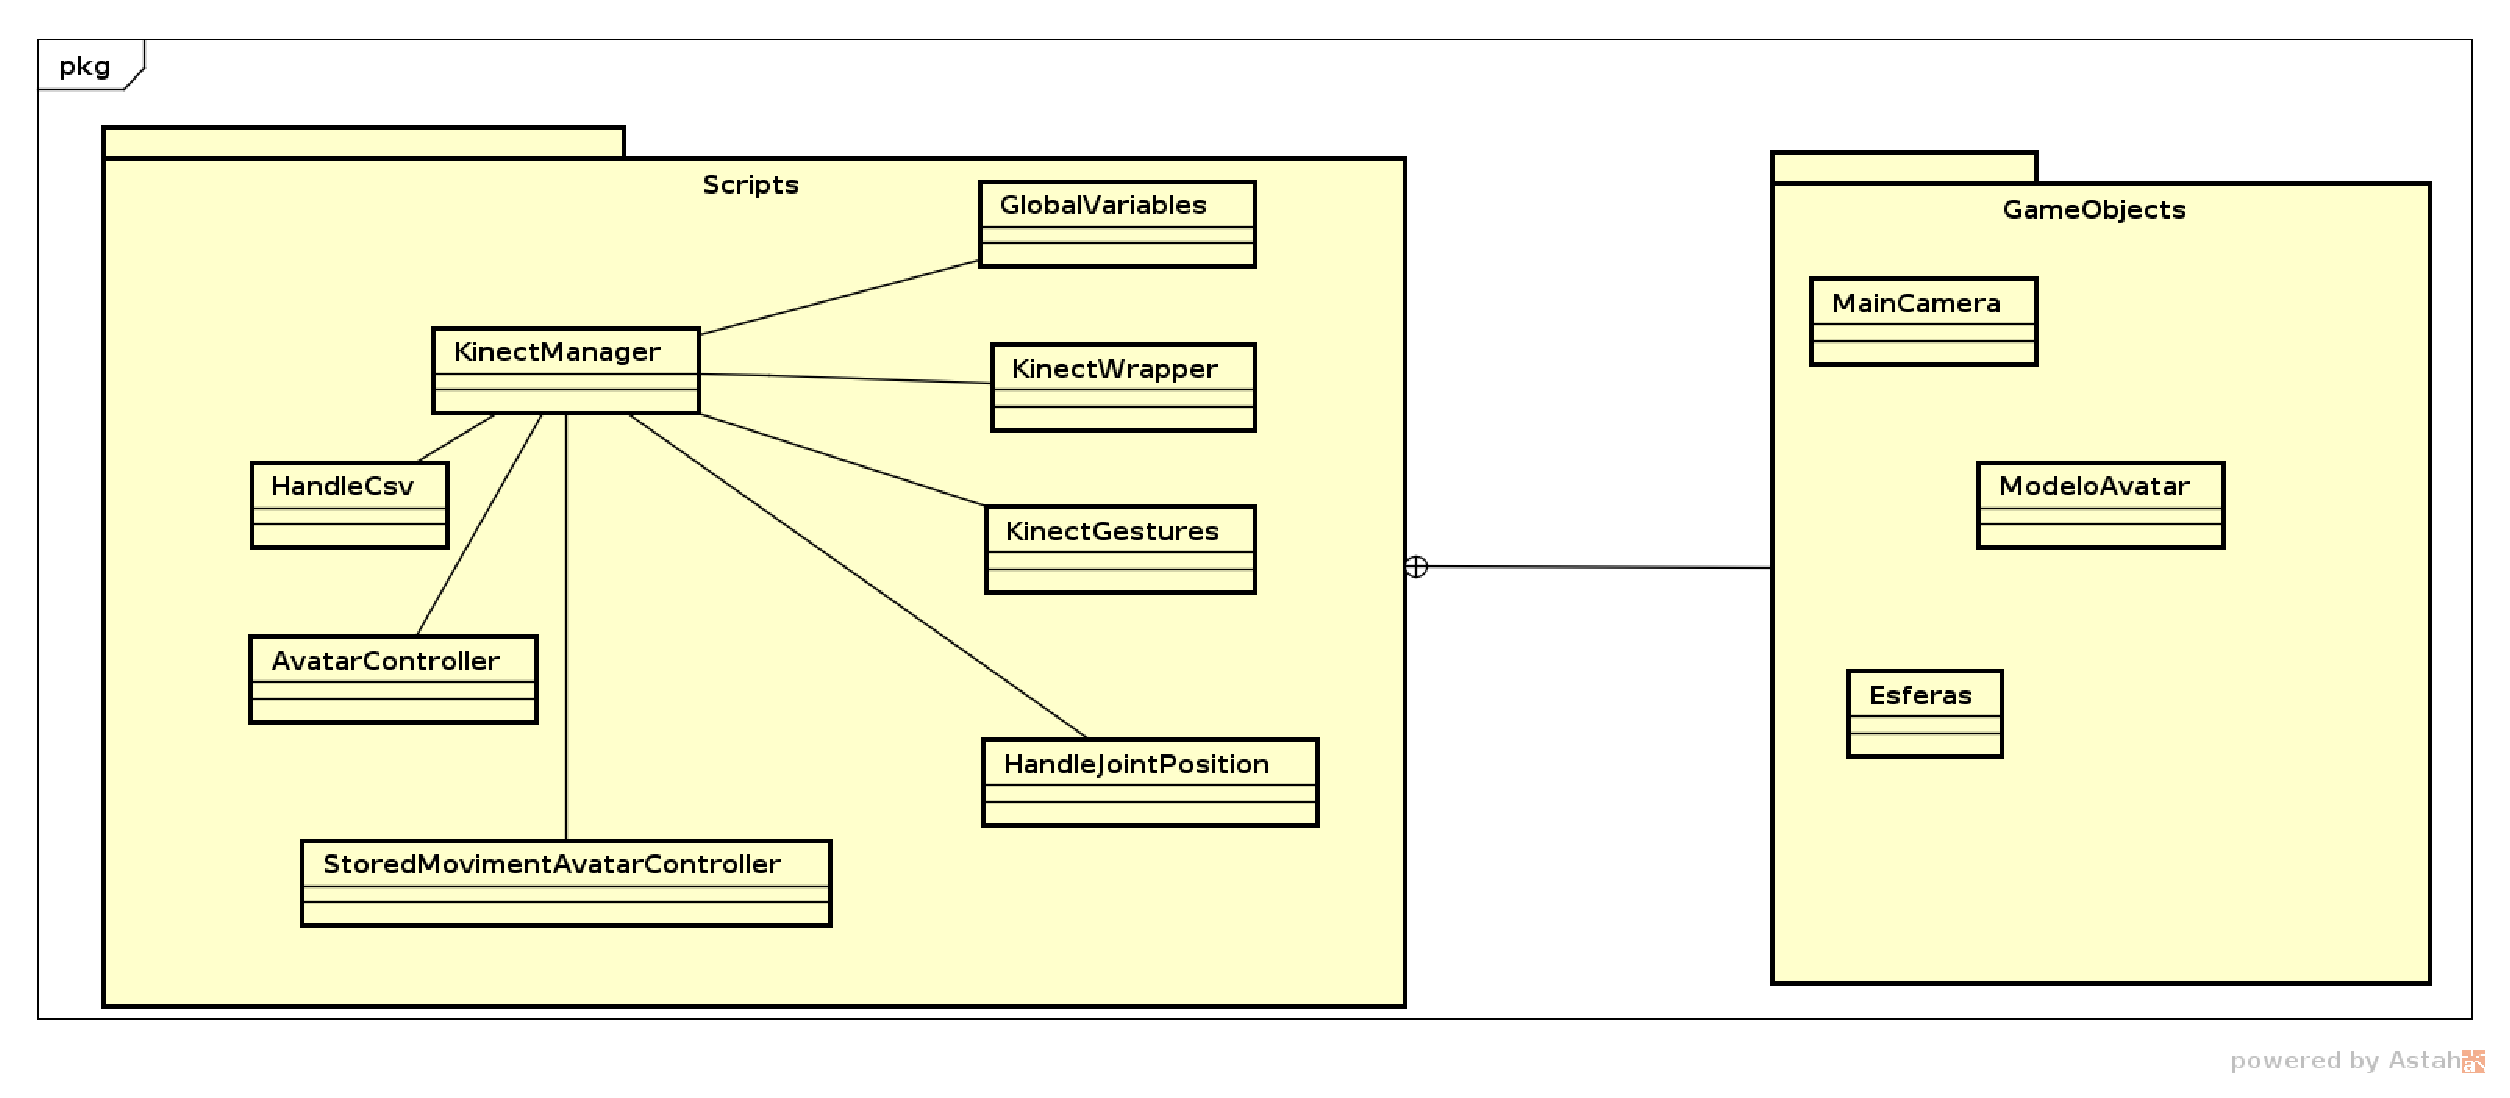
\includegraphics [keepaspectratio=true,scale=0.45]{figuras/DiagramaDeClasse.eps}

  \caption{Diagrama de classe referente ao sistema}
  \label{diagramaClasse}
  \end{figure}

  Abaixo vemos uma representação da sequência de mensagens do sistema.


      \begin{figure}[H]
      \centering
      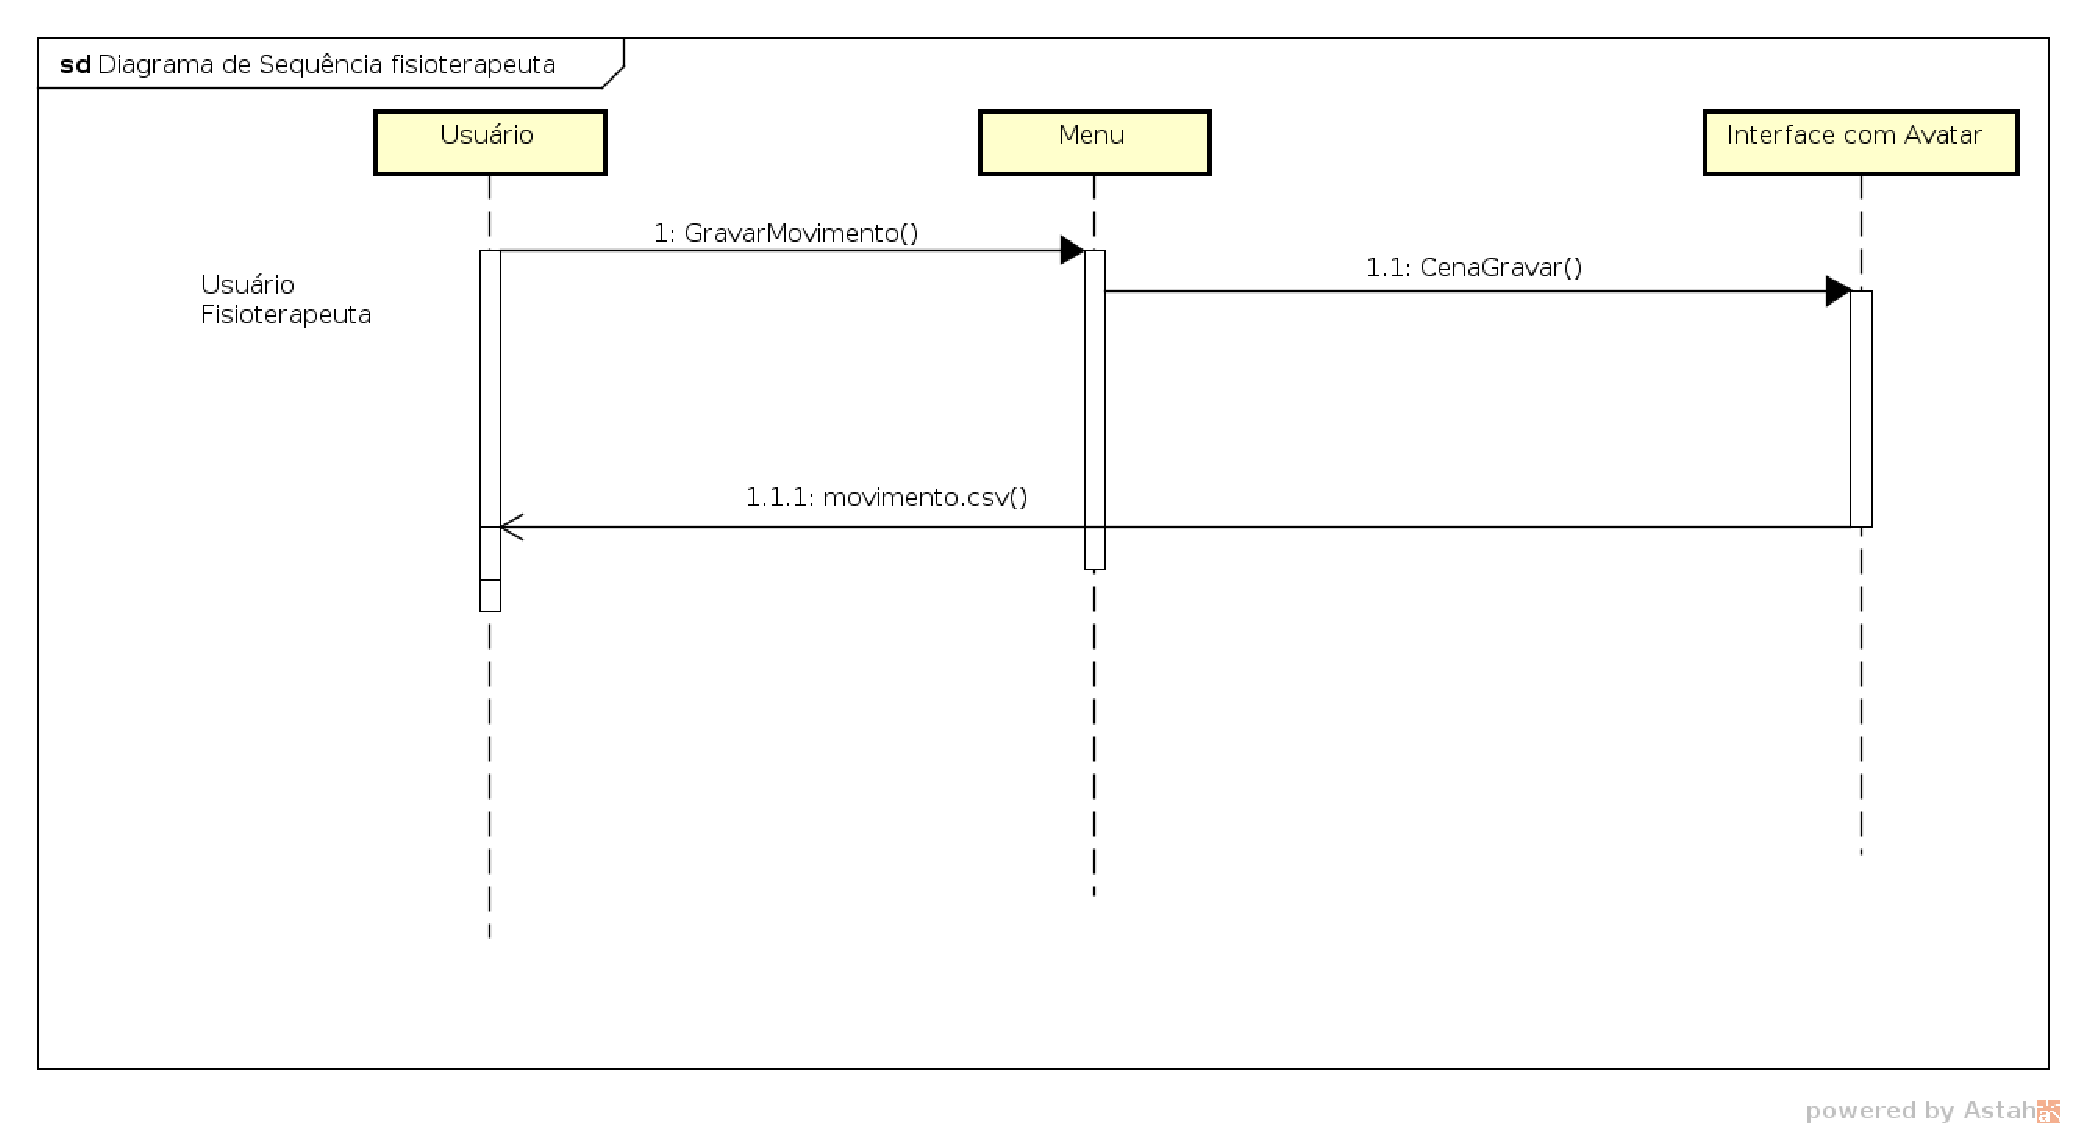
\includegraphics [keepaspectratio=true,scale=0.45]{figuras/diagramaFisio.eps}

      \caption{Diagrama de sequência referente ao uso do fisioterapeuta}
      \label{diagramaFisio}
      \end{figure}


      \begin{figure}[H]
      \centering
      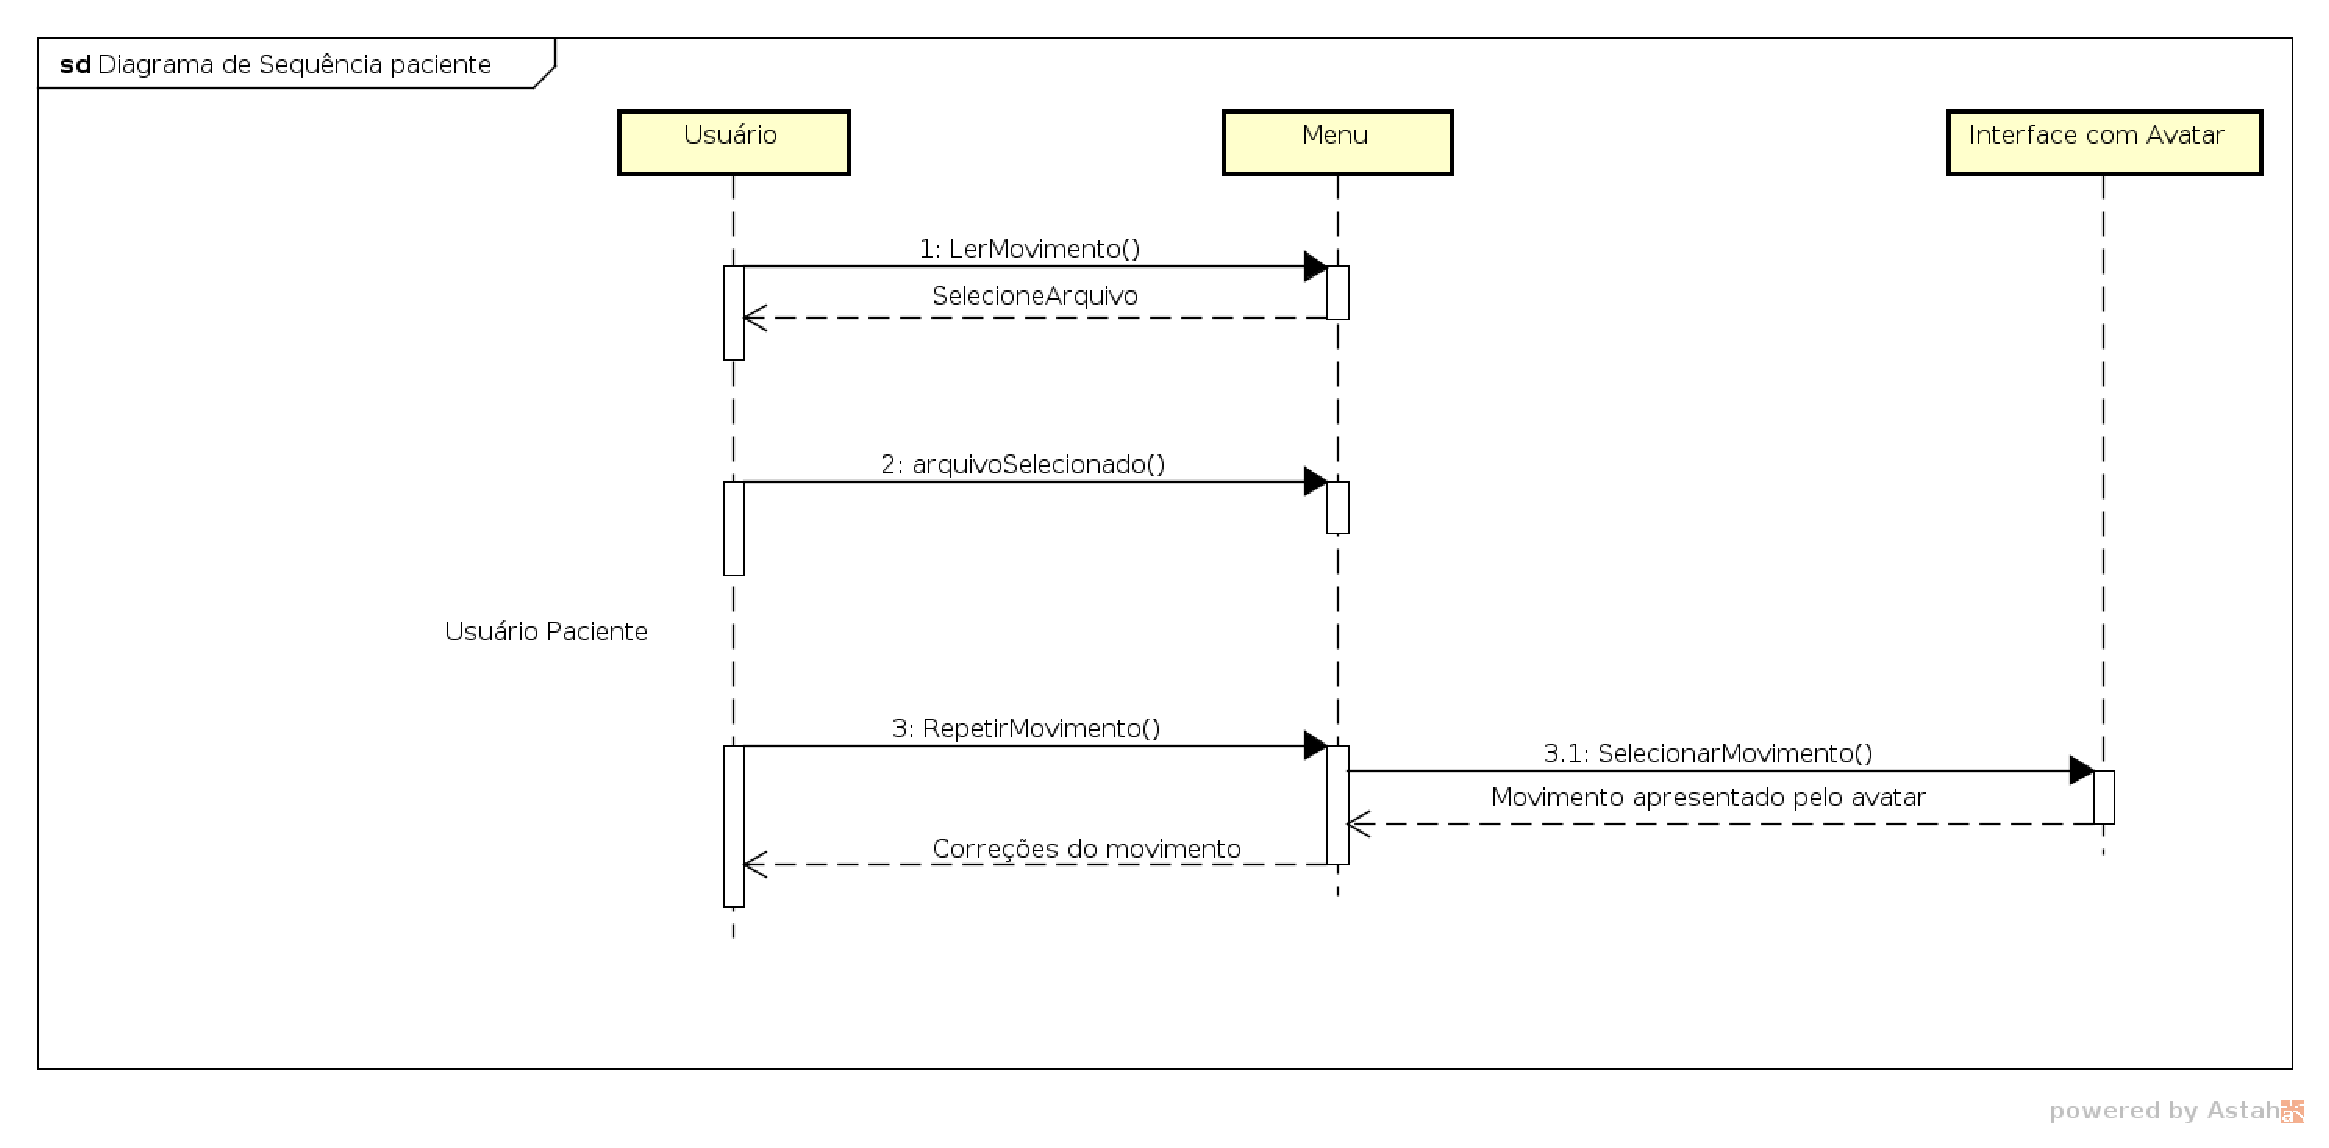
\includegraphics [keepaspectratio=true,scale=0.45]{figuras/diagramaPaciente.eps}

      \caption{Diagrama de sequência referente ao uso do paciente}
      \label{diagramaPaciente}
      \end{figure}



  A arquitetura dos scripts, ficou um pouco focada na classe \textit{KinectManager}, pois ela é a responsável pela comunicação com o kinect.
Nas próximas seções, falaremos um pouco sobre o papel de cada classe.

\subsection{\textit{KinectManager}}\label{sub:kmanager}
  Classe implementada em C\# e tem como principal responsabilidade gerir a comunicação com o kinect. Com a ajuda da classe \textit{KinectWrapper}(\ref{sub:kwrapper}), ela
  abstrai as funções, estruturas e recursos do Kinect. Esta classe possui várias funções, abaixo descrevemos as principais:

  \begin{itemize}
      \item \textit{\textbf{ProcessSkeleton()}}: Processa os dados do "esqueleto", dados sobre as posições e rotações das juntas do usuário;
      \item \textit{\textbf{HandlejointPosition()}}: Pega os dados sobre as posições das juntas para animação do avatar 3d;

  \end{itemize}

\subsection{\textit{HandletCsv}}\label{sub:getcsv}
  Classe implementada em C\# e tem como principal responsabilidade fazer o parser do arquivo csv do movimento desejado. Abaixo descrevemos sua principal função:

  \begin{itemize}
      \item \textit{\textbf{getSkeletonPositionFromCSV()}}: Processa os dados do "esqueleto" no arquivo, estruturando essas informações em uma matriz de float.
  \end{itemize}

\subsection{\textit{AvatarController}}\label{sub:avatarc}
  Classe implementada em C\# e tem como principal responsabilidade animar o avatar 3d de acordo com a movimentação do usuário em tempo real. Com a ajuda da classe \textit{KinectManager}(\ref{sub:kmanager}), ela
  converte a posição das juntas para animação do avatar. Esta classe possui várias funções, abaixo descrevemos as principais:

  \begin{itemize}
      \item \textit{\textbf{UpdateAvatar()}}: Processa os dados das juntas do usuário, convertendo essas informações por frame para animação 3d;
      \item \textit{\textbf{TransformBone()}}: Aplica as rotações monitoradas pelo \textit{kinect} para as juntas do avatar.;

  \end{itemize}

  \subsection{\textit{StoredMovimentAvatarController}}\label{sub:storedavatarc}
    Classe implementada em C\# e tem como principal responsabilidade movimentar o avatar, porém de acordo com o movimento parseado. Além de possuir as mesmas funções da
  \textit{AvatarController}(\ref{sub:avatarc}), essa classe também é a responsável de fazer a comparação do movimento do usuário com o movimento salvo. A principal função
  responsável por fazer esta comparação é a \textit{CalculeAngle()}, que espera como argumento a posição de três juntas interligadas ( três vetores -\textit{Vector3}) e retorna o ângulo entre elas.

  \subsection{\textit{GetJointPosition}}\label{sub:getjoint}
    Classe implementada em C\# e tem como principal responsabilidade escrever as posições de todas as juntas e exportar para csv. Com a ajuda da classe \textit{KinectManager}(\ref{sub:kmanager}),
    ela captura os dados sobre as juntas do usuário. Abaixo descrevemos sua principal função:

    \begin{itemize}
        \item \textit{\textbf{Update()}}: Processa os dados do "esqueleto" e escreve no arquivo csv a cada frame.
    \end{itemize}

  \subsection{\textit{KinectGesture}}\label{sub:kgesture}
    Classe implementada em C\# e tem como principal responsabilidade a identificação de gestos já mapeados.

  \subsection{\textit{KinectWrapper}}\label{sub:kwrapper}
    Classe implementada em C\# e tem como principal responsabilidade deter as várias estruturas e importações dll. É esta classe que abstrai a comunicação com o
    \textit{SDK}(\ref{sub:sdk}).

  \subsection{\textit{GlobalVariables}}\label{sub:gvariable}
    Classe implementada em C\# e tem como principal responsabilidade guardar as informações dos movimentos parseados.


  \subsection{Requisitos do sistema}\label{sec:requisitosSistema}
   Esta seção apresentará os requisitos do sistema:
   \begin{itemize}
   \item \textbf{Funcionalidade}(Functionality):
     \begin{itemize}
     \item Captura do movimento do usuário pelo sistema (leitura dos ângulos das articulações);
     \item Importação de movimento;
     \item Apresentação de uma lista de movimentos gravados para seleção e execução;
     \item Animação do avatar com o movimento correto;
     \item Comparação das articulações de referência com os realizados pelo usuário;
     \item Exibição no avatar 3d as discrepâncias entre o movimento desejado e o movimento realizado.
     \end{itemize}
   \item \textbf{Usabilidade}(Usability)
     \begin{itemize}
     \item O usuário do sistema será capaz de visualizar todo tipo de informação
      textual, imagem ou modelo 3d na aplicação , com clareza, em qualquer
     monitor independente de resolução.
     %\item Documentação ampla e de fácil compreensão, abordando todas as
     %funcionalidades disponível na aplicação.
     \end{itemize}
  \item \textbf{Confiabilidade}(Reability)
     \begin{itemize}
     \item O sistema será capaz de verificar algum erro ou inconstância entre os
      dados recebidos dos sensores, podendo assim se recuperar ou informar
     alguma falha na comunicação com os mesmos.
     \end{itemize}
  \item \textbf{Desempenho}(Performance)
     \begin{itemize}
     \item O sistema analisará o movimento feito pelo usuário em streaming.
     \end{itemize}
  \item \textbf{Suportabilidade}(Supportability)
     \begin{itemize}
     \item Em sua versão inicial será exclusivo do sistema operacional da microsoft, o windows, podendo ser executado nas versões 7,8 e 10.
     \end{itemize}
   \end{itemize}



\section{Configuração e Integração das Tecnologias}
Nesta seção, são apresentados o passo a passo para a configuração e integração das tecnologias utilizadas durante o desenvolvimento do sistema,
incluindo a etapa de configuração do ambiente de programação e
do ambiente para a utilização do kinect, assim podendo ser aplicada e analisada por outros interessados.

\subsection{Instalação do SDK}
  Primeiramente, para possibilitar a comunicação entre o PC e o kinect, deve-se
instalar o SDK 1.8, o qual pode ser encontrado \href{https://www.microsoft.com/en-us/download/details.aspx?id=40278}{aqui}\footnote{https://www.microsoft.com/en-us/download/details.aspx?id=40278}.
  Lembrando que o kinect é feito para console, não é comum computadores darem suporte para o formato do
cabo, sendo assim para comunicar o PC e Kinect será preciso de uma fonte para Kinect Xbox 360.
  Depois do sdk instalado, conecte o Kinect na fonte e a fonte no PC. Para verificar se seu sitema operacional
está comunicando com o sensor alguns passos devem ser seguidos:

\begin{enumerate}
  \item Clicar em iniciar
  \item Ir em Meu computador
  \item Clicar com o botão direito
  \item Clicar em propriedades
  \item Na janela que foi aberta, ir em Gerenciador de dispositivos
  \item Verificar se na lista de dispositivos se encontra "Kinect for Windows" exibido como na imagem abaixo.
\end{enumerate}


\begin{figure}[H]
\centering
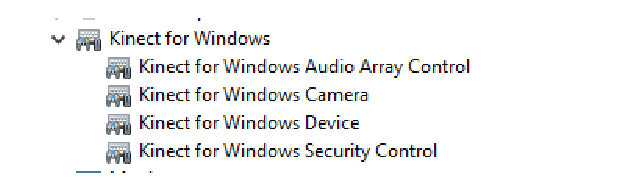
\includegraphics [keepaspectratio=true,scale=0.60]{figuras/gerenciadorDispositivo.eps}

\caption{Gerenciador de Dispositivo}
\label{gerenciadorDispositivo}
\end{figure}

\subsection{Instalação do Unity 3d}\label{sub:instalacaoUnity}
  Como já dito no capítulo Suporte Tecnológico(\ref{ch:suporteTecnologico}), o Unity 3d é um motor gráfico, criado para jogos em três dimensões e duas dimensões,
sendo a principal tecnologia usado para o desenvolvimento do sistema, para cálculos das juntas e para o \textit{feedback} ao usuário.
O Unity 3d pode ser encontrado \href{https://unity3d.com/pt/get-unity/download}{aqui}\footnote{https://unity3d.com/pt/get-unity/download}.

  Ao instalar o unity 3d, o instalador dará
a opção de instalar o visual studio mais recente, é aconselhável aceitar pois este é um editor de texto com várias funções para a edição
de arquivos C\#.

\subsection{Utilizando o Unity 3d}
  Após a instalação de ambas as tecnologias, na primeira vez em que se abre o unity 3d é necessário fazer um cadastro para sua utilização. Feito
o cadastro:
\begin{enumerate}
  \item Na primeira janela do unity 3d é perguntado se deseja criar um novo projeto ou importar, clique em importar
  \item Procure o local onde se encontra a pasta do projeto e importe.
\end{enumerate}

  Pronto, agora será possível mexer no projeto pelo unity 3d. Para abrir o projeto no visual studio é somente clicar com o botão direito em cima
da cena desejada e clicar em "\textit{Open C\# Project}".

\subsection{Histórias de usuário do sistema}
\label{sec:Histórias de usuário}
  Como prática ágil as \textit{User stories} (Histórias de usuário), são artefatos
de desenvolvimento, utilizadas para organizar requisitos. Tem-se foco nos objetivos
do usuário e como o sistema alcança esses objetivos.

  Para melhor organizar e fracionar os requisitos deste trabalho, foi adotado
essa prática ágil, podemos ver o levantamento das histórias de usuário na tabela Histórias(\ref{historias}).
\begin{table}[H]
\centering
\caption{Histórias}
\label{historias}
\begin{tabular}{|l|l|}
\hline
\textbf{História} & 1                                                        \\ \hline
\textbf{Eu como}  & Fisioterapeuta                    \\ \hline
\textbf{Desejo}   & Que o sistema mapeie meu movimento sendo executado corretatmente                   \\ \hline
\textbf{Para}     & poder comparar com o movimento do paciente \\ \hline
 \multicolumn{2}{|l|}{}                                                       \\ \hline
\textbf{História} & 2                                                        \\ \hline
\textbf{Eu como}  & Usuário                                    \\ \hline
\textbf{Desejo}   & Poder carregar movimento previamente mapeado                \\ \hline
\textbf{Para}     & Constar no menu do sistema\\ \hline
\multicolumn{2}{|l|}{}                                                       \\ \hline
\textbf{História} & 3                                                        \\ \hline
\textbf{Eu como}  & Fisioterapeuta                    \\ \hline
\textbf{Desejo}   & Que o sistema salve um novo movimento                    \\ \hline
\textbf{Para}     & Poder constar no menu do sistema e poder ser executado \\ \hline
\multicolumn{2}{|l|}{}                                                       \\ \hline
\textbf{História} & 4                                                        \\ \hline
\textbf{Eu como}  & Usuário                                                  \\ \hline
\textbf{Desejo}   & Desejo escolher movimento de referência                  \\ \hline
\textbf{Para}     & Melhor seguir receita médica                             \\ \hline
\multicolumn{2}{|l|}{}                                                       \\ \hline

\textbf{História} & 5                                                        \\ \hline
\textbf{Eu como}  & Usuário                                                  \\ \hline
\textbf{Desejo}   & Feedback do movimento sendo executado em tempo real                    \\ \hline
\textbf{Para}     & Poder melhor executar os movimentos das articulações           \\ \hline
\multicolumn{2}{|l|}{}                                                       \\ \hline

\end{tabular}
\end{table}

  Tais histórias compões as funcionalidades do sistema(\ref{sub:features}) e foram implementadas no Unity 3d.


 \section{Funcionalidades do sistema - \textit{features}}\label{sub:features}
     As \textit{features} no desenvolvimento ágil é um pedaço de funcionalidade que oferece valor comercial \cite{versionOne}.
   Geralmente as \textit{features} tem uma granularidade maior que as \textit{User Stories}(Histórias de usuário~\ref{sec:Histórias de usuário}).
   Podemos dizer que algumas features são compostas de \textit{User Stories}.

     O sistema possui três features, gravação de movimento, leitura de arquivo do movimento desejado e análise da repetição do movimento:
   \begin{enumerate}
     \item \textbf{Gravar movimento:} Essa funcionalidade permite a gravação do movimento, deve ser feito pelo profissional fisioterapeuta
     para uma correta execução. Será esse movimento que o sistema usará como gabarito. O sistema retorna um arquivo csv. Podemos observar essa funcionalidade
     na tela do sistema em \ref{img:gravarmovimento}.

     \item \textbf{Ler arquivo de movimento:} Essa funcionalidade espera um arquivo csv e armazena o movimento no sistema.Podemos observar essa funcionalidade
     na tela do sistema em \ref{img:lerArquivo}.

     \item \textbf{Praticar movimento:} Essa funcionalidade mostra a correta execução do movimento e analisa com o movimento do paciente.Podemos observar essa funcionalidade
     na tela do sistema em \ref{img:praticarMovimento}.

   \end{enumerate}

   Como observado na imagem \ref{img:menu}, podemos visualizar todas as funcionalidades a partir do menu do sistema.

   \begin{figure}[H]
   \centering
   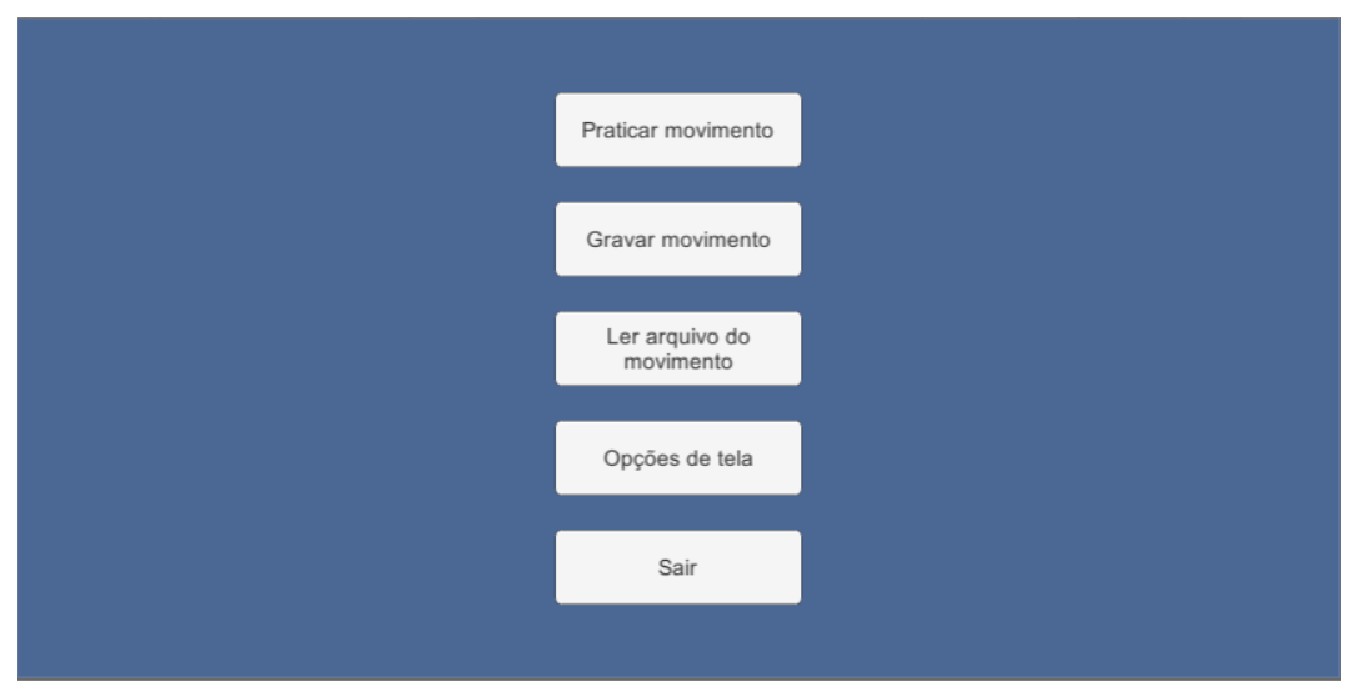
\includegraphics [keepaspectratio=true,scale=0.40]{figuras/menu.eps}
   \caption{Menu do sistema}
   \label{img:menu}
   \end{figure}

     Abaixo será listado as telas do sistema relacionado as três funcionalidades

     \begin{figure}[H]
     \centering
     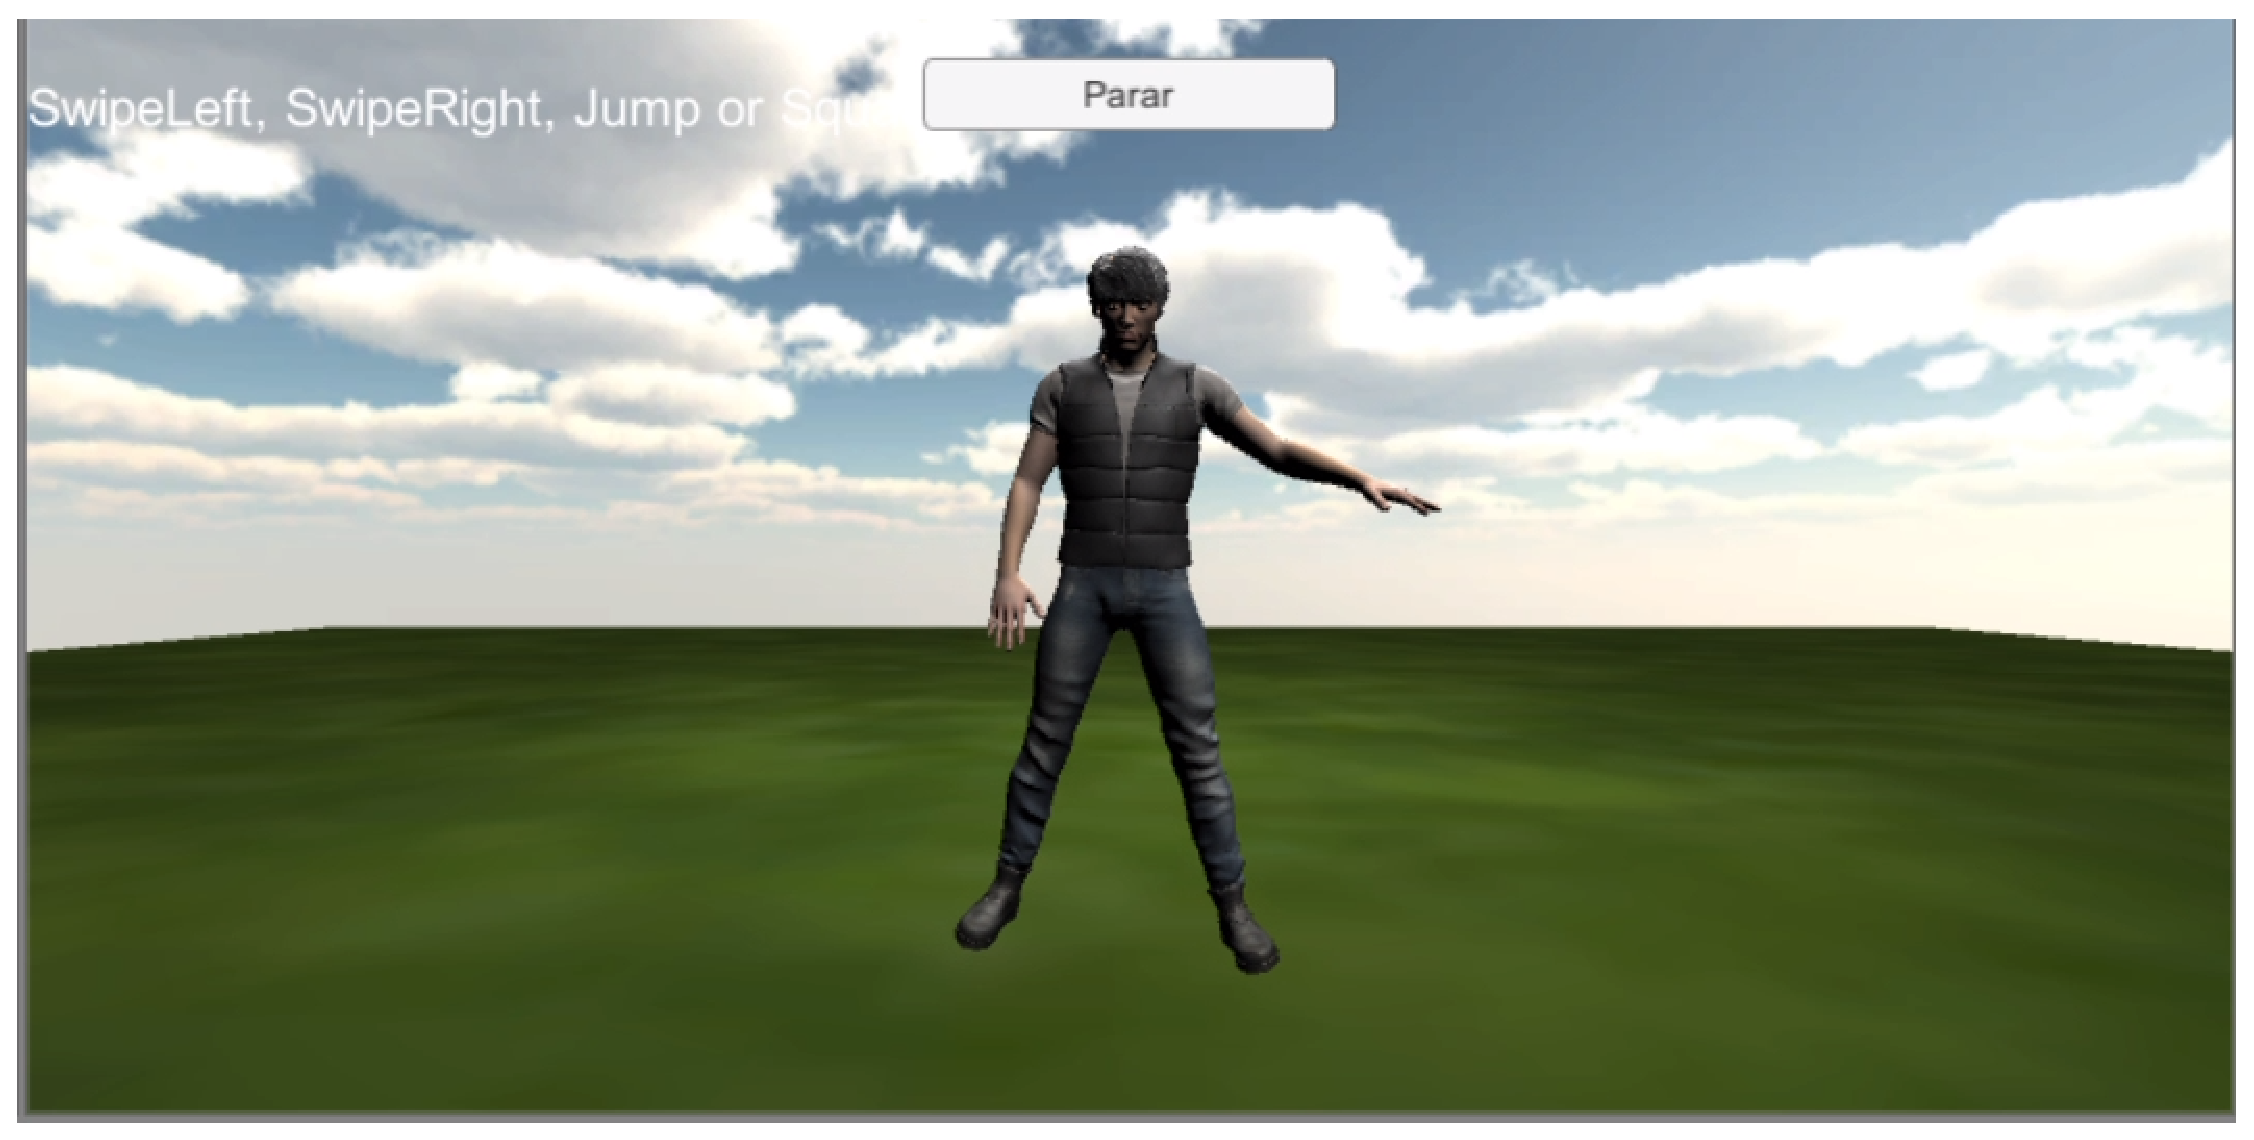
\includegraphics [keepaspectratio=true,scale=0.40]{figuras/gravarmovimento.eps}
     \caption{Gravar movimento}
     \label{img:gravarmovimento}
     \end{figure}

     \begin{figure}[H]
     \centering
     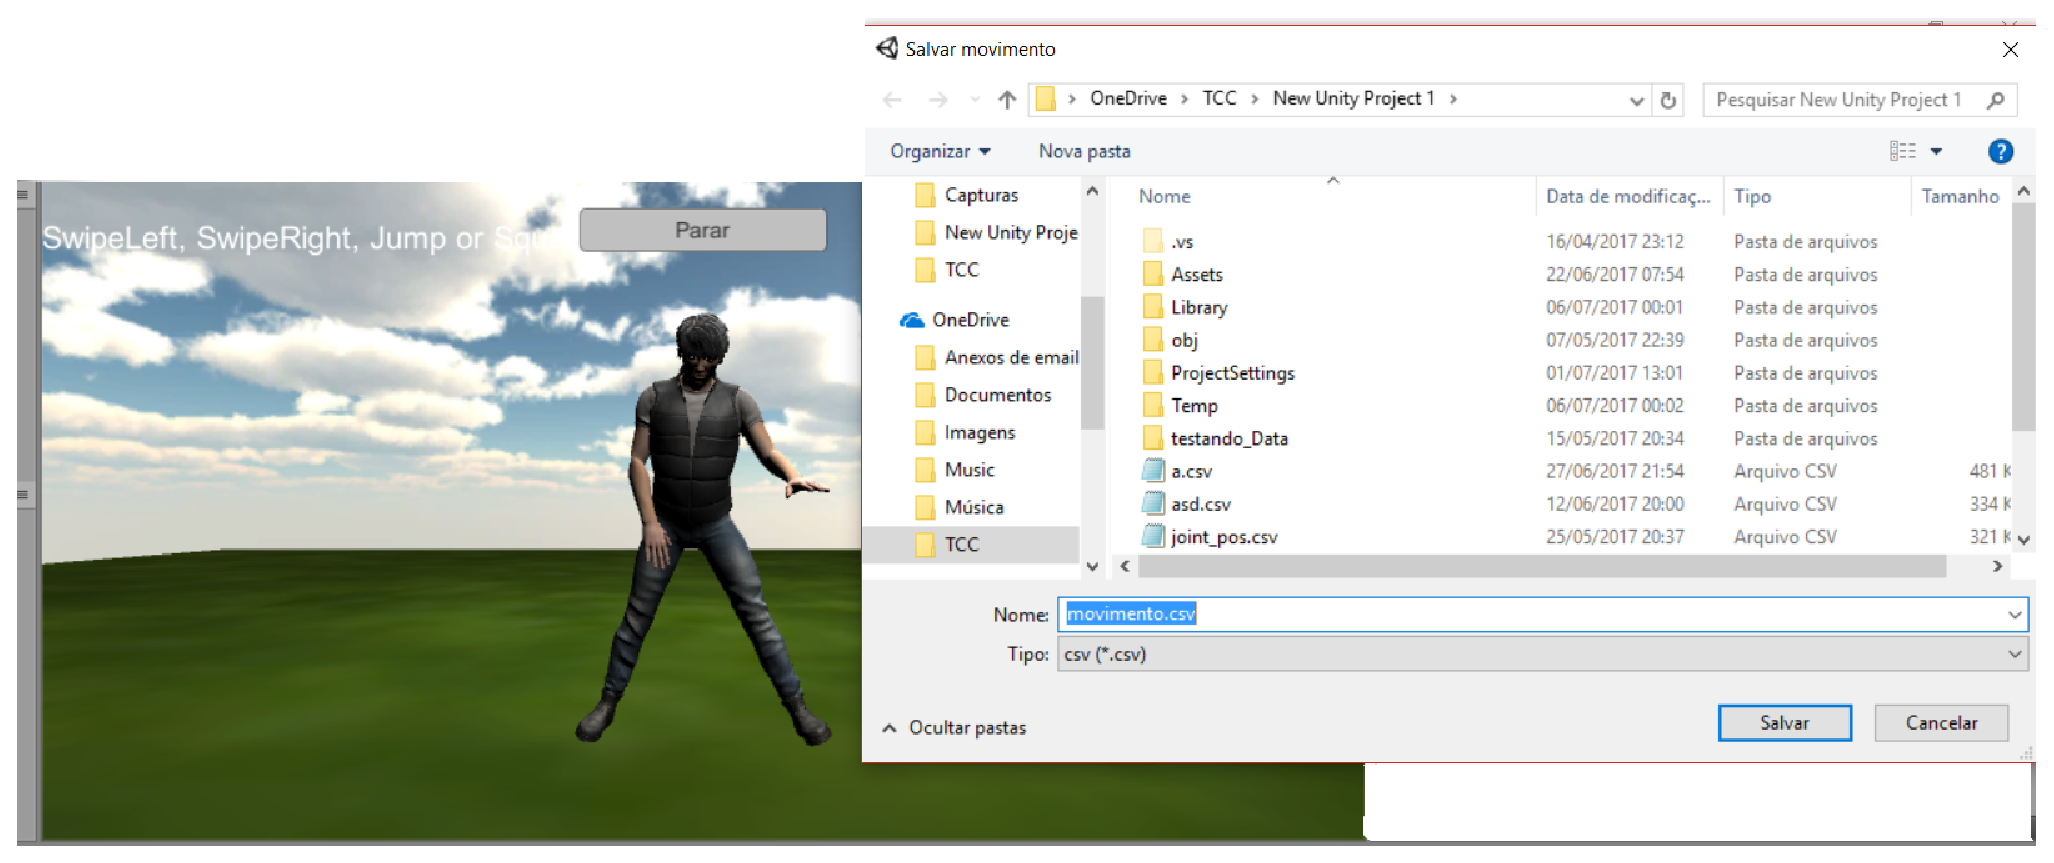
\includegraphics [keepaspectratio=true,scale=0.40]{figuras/gravarmovimento2.eps}
     \caption{Gravar movimento}
     \label{img2:gravarmovimento}
     \end{figure}

     \begin{figure}[H]
     \centering
     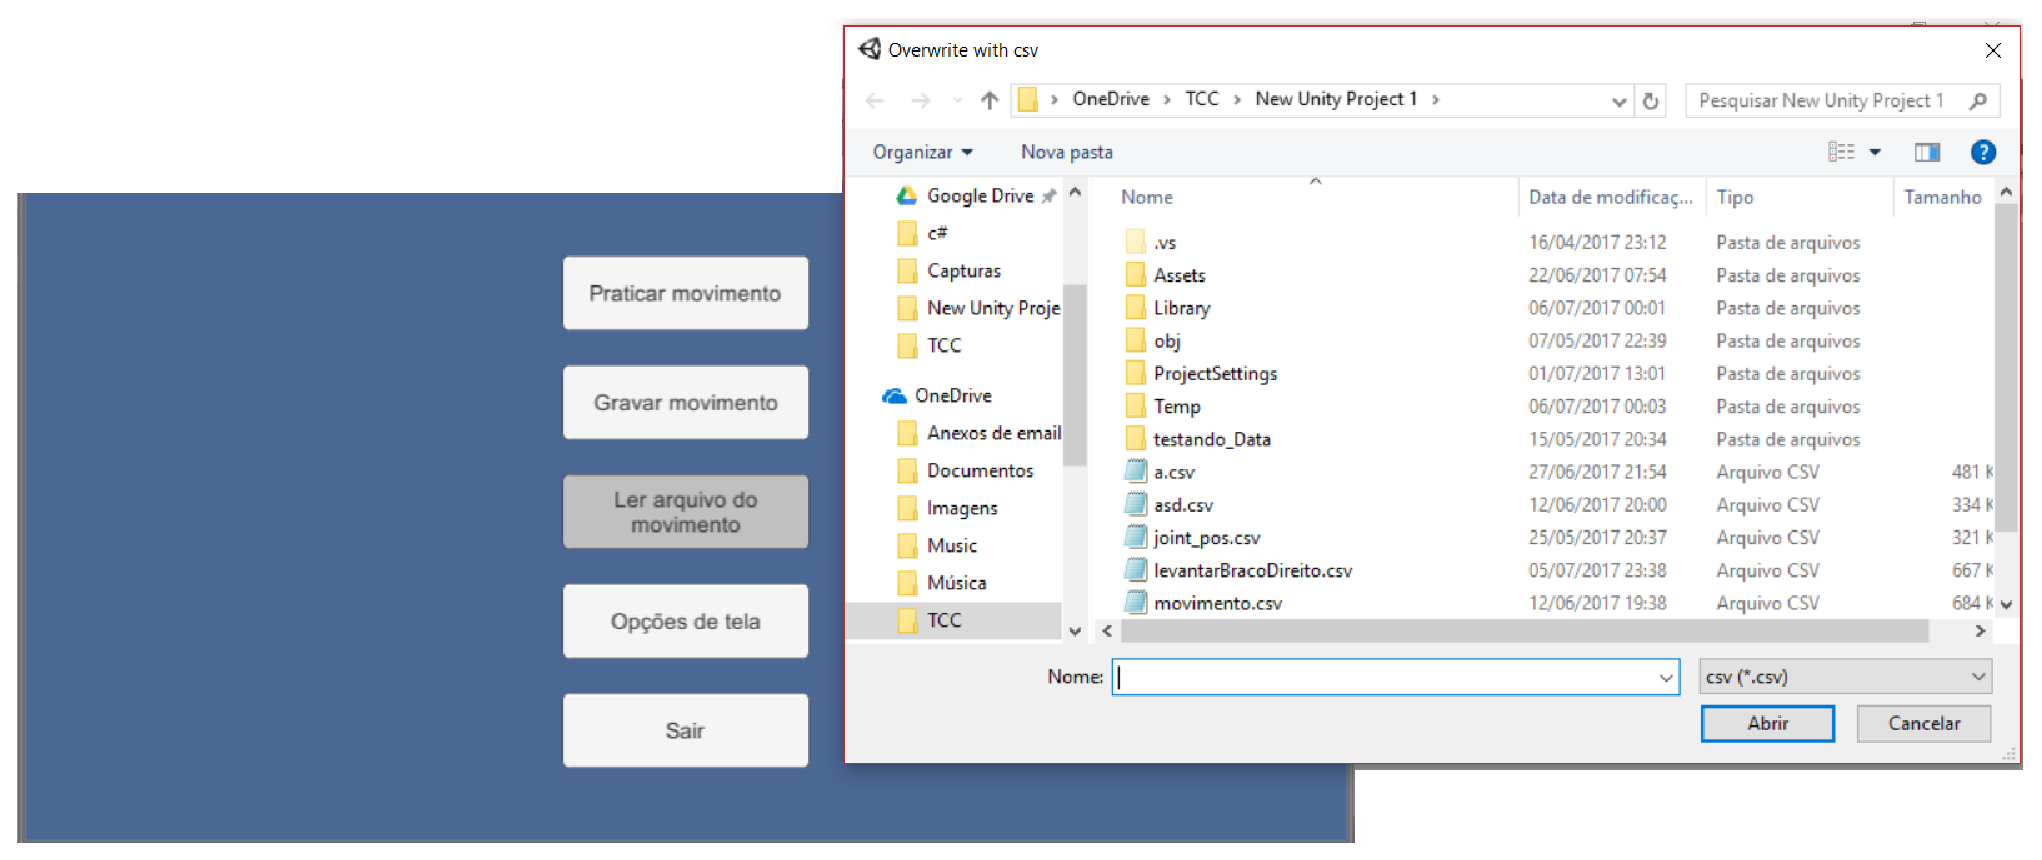
\includegraphics [keepaspectratio=true,scale=0.40]{figuras/lerarquivo.eps}
     \caption{Ler Arquivo de Movimento}
     \label{img:lerArquivo}
     \end{figure}

     \begin{figure}[H]
     \centering
     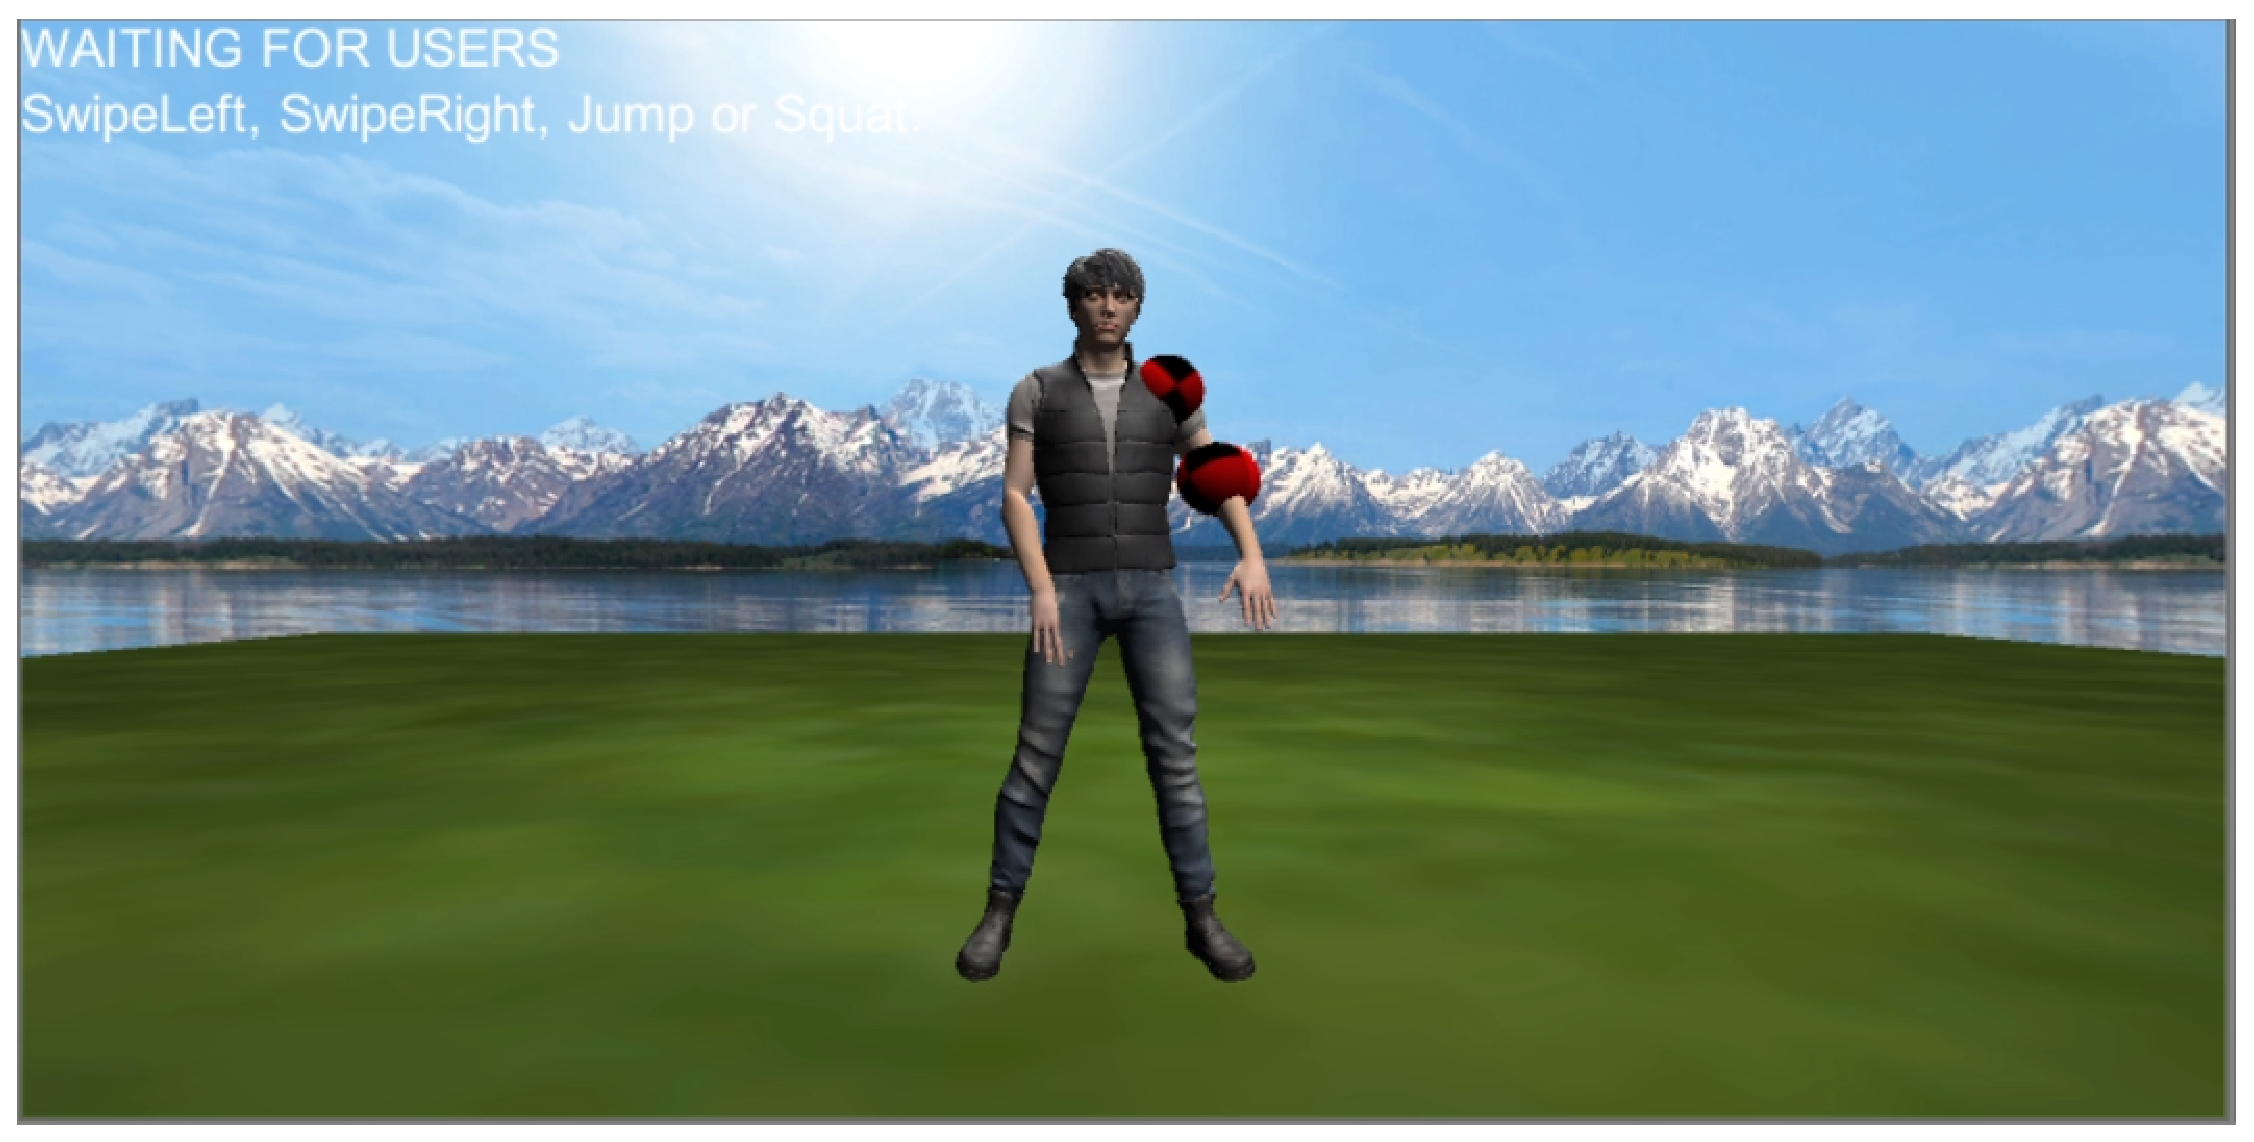
\includegraphics [keepaspectratio=true,scale=0.40]{figuras/praticarmovimento.eps}
     \caption{Praticar Movimento}
     \label{img:praticarMovimento}
     \end{figure}

     \begin{figure}[H]
     \centering
     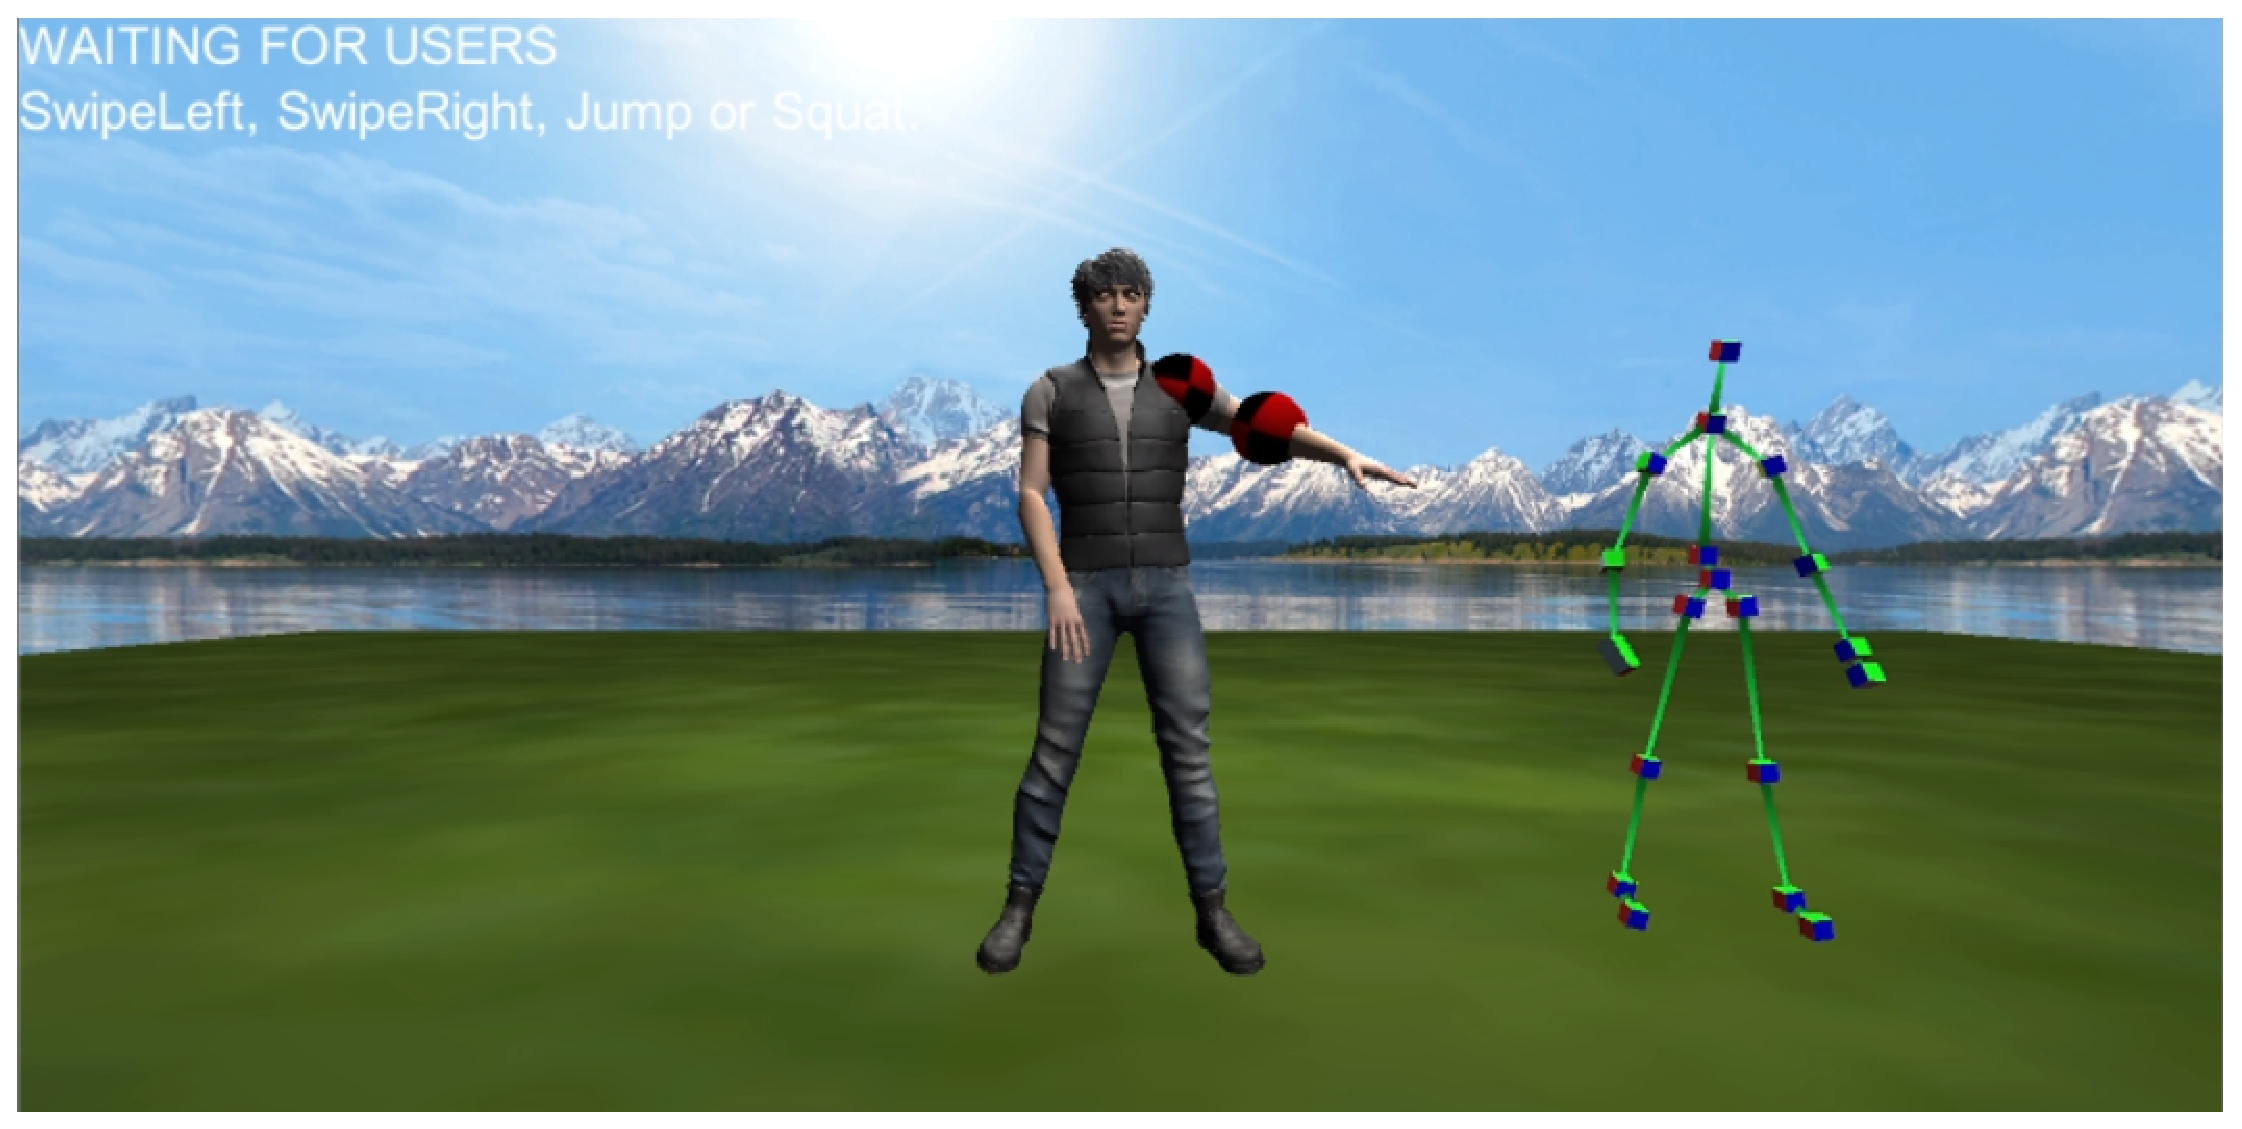
\includegraphics [keepaspectratio=true,scale=0.40]{figuras/praticarmovimento2.eps}
     \caption{Praticar Movimento com esqueleto para auxílio ao desenvolvimento}
     \label{img2:praticarMovimento}
     \end{figure}


   Podemos ver o detalhamento das features em Histórias de usuário do sistema(\ref{historias}).
